\documentclass[margin=2mm]{standalone}
\usepackage{tikz}
\usepackage{amsmath,amssymb,mathtools}
\begin{document}
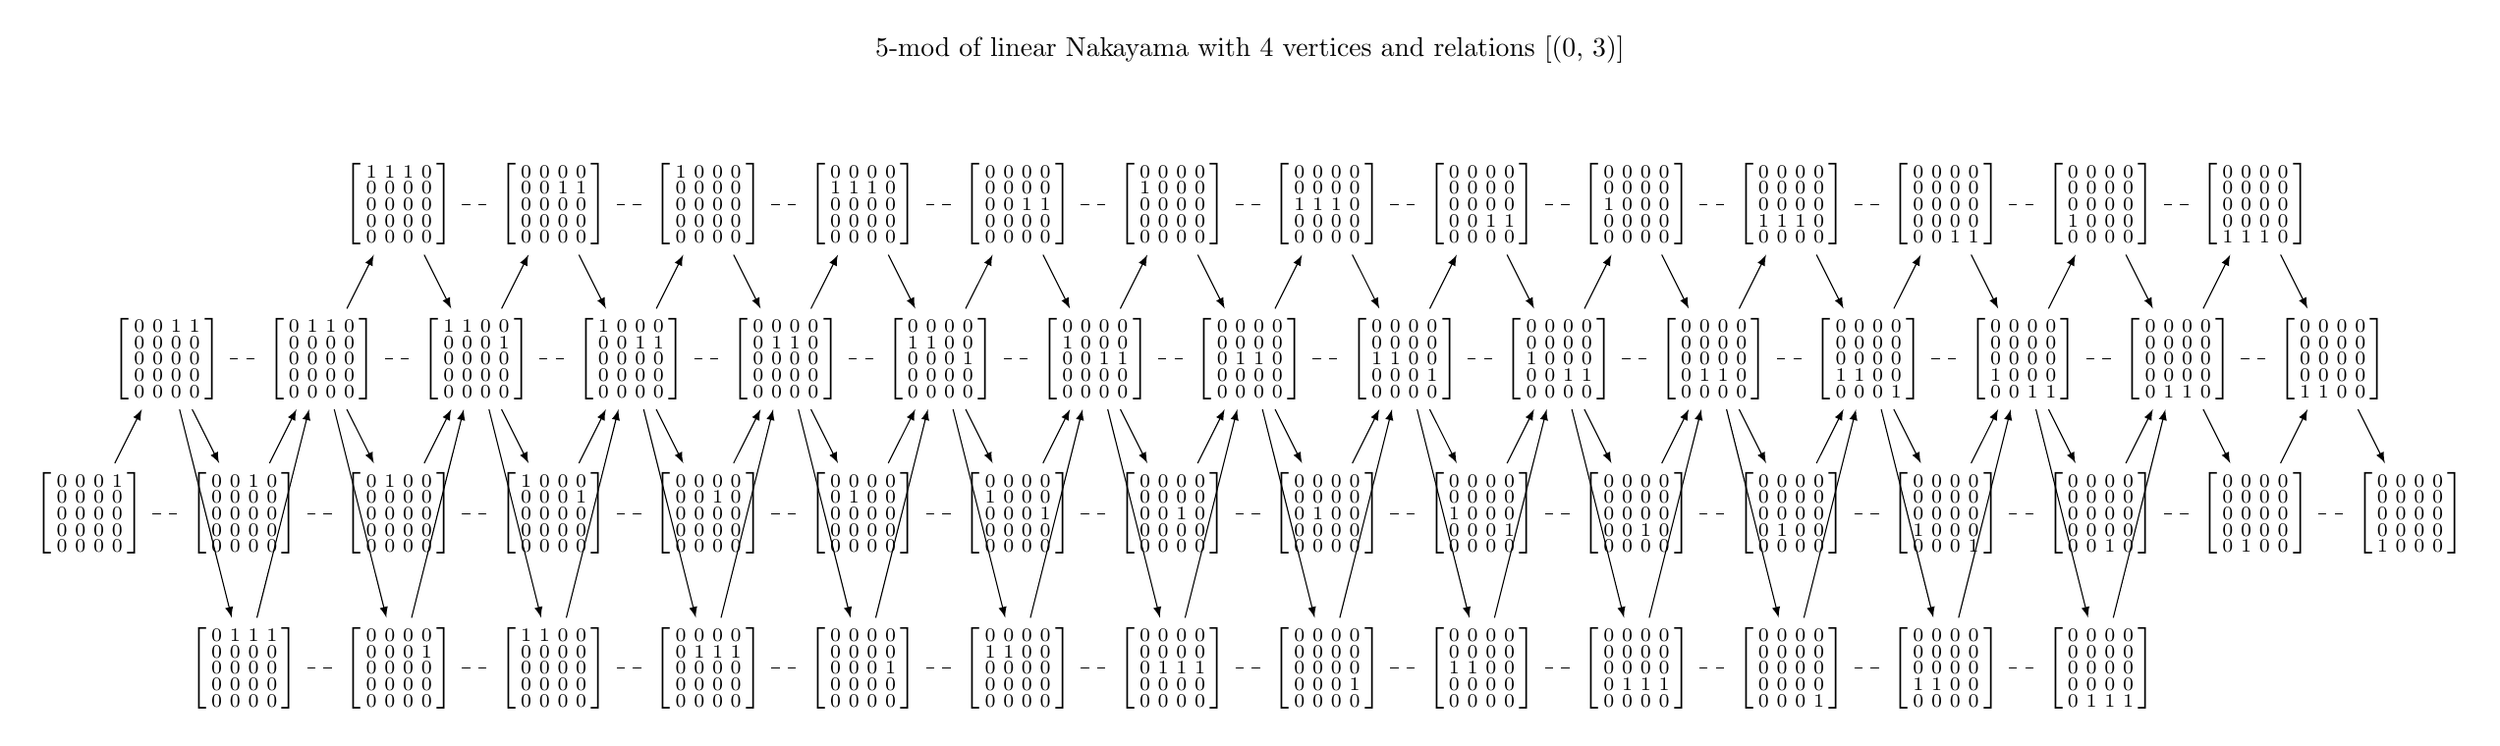
\begin{tikzpicture}[xscale=1,yscale=2]
\node at (15.0,3) [] {$5$-mod of linear Nakayama with 4 vertices and relations [(0, 3)]};
\node (t-0P0) at (4,2) [scale=1] {$\begin{bsmallmatrix}
 1 & 1 & 1 & 0\\
 0 & 0 & 0 & 0\\
 0 & 0 & 0 & 0\\
 0 & 0 & 0 & 0\\
 0 & 0 & 0 & 0\\
\end{bsmallmatrix}$};
\node (t-1P0) at (6,2) [scale=1] {$\begin{bsmallmatrix}
 0 & 0 & 0 & 0\\
 0 & 0 & 1 & 1\\
 0 & 0 & 0 & 0\\
 0 & 0 & 0 & 0\\
 0 & 0 & 0 & 0\\
\end{bsmallmatrix}$};
\node (t-2P0) at (8,2) [scale=1] {$\begin{bsmallmatrix}
 1 & 0 & 0 & 0\\
 0 & 0 & 0 & 0\\
 0 & 0 & 0 & 0\\
 0 & 0 & 0 & 0\\
 0 & 0 & 0 & 0\\
\end{bsmallmatrix}$};
\node (t-3P0) at (10,2) [scale=1] {$\begin{bsmallmatrix}
 0 & 0 & 0 & 0\\
 1 & 1 & 1 & 0\\
 0 & 0 & 0 & 0\\
 0 & 0 & 0 & 0\\
 0 & 0 & 0 & 0\\
\end{bsmallmatrix}$};
\node (t-4P0) at (12,2) [scale=1] {$\begin{bsmallmatrix}
 0 & 0 & 0 & 0\\
 0 & 0 & 0 & 0\\
 0 & 0 & 1 & 1\\
 0 & 0 & 0 & 0\\
 0 & 0 & 0 & 0\\
\end{bsmallmatrix}$};
\node (t-5P0) at (14,2) [scale=1] {$\begin{bsmallmatrix}
 0 & 0 & 0 & 0\\
 1 & 0 & 0 & 0\\
 0 & 0 & 0 & 0\\
 0 & 0 & 0 & 0\\
 0 & 0 & 0 & 0\\
\end{bsmallmatrix}$};
\node (t-6P0) at (16,2) [scale=1] {$\begin{bsmallmatrix}
 0 & 0 & 0 & 0\\
 0 & 0 & 0 & 0\\
 1 & 1 & 1 & 0\\
 0 & 0 & 0 & 0\\
 0 & 0 & 0 & 0\\
\end{bsmallmatrix}$};
\node (t-7P0) at (18,2) [scale=1] {$\begin{bsmallmatrix}
 0 & 0 & 0 & 0\\
 0 & 0 & 0 & 0\\
 0 & 0 & 0 & 0\\
 0 & 0 & 1 & 1\\
 0 & 0 & 0 & 0\\
\end{bsmallmatrix}$};
\node (t-8P0) at (20,2) [scale=1] {$\begin{bsmallmatrix}
 0 & 0 & 0 & 0\\
 0 & 0 & 0 & 0\\
 1 & 0 & 0 & 0\\
 0 & 0 & 0 & 0\\
 0 & 0 & 0 & 0\\
\end{bsmallmatrix}$};
\node (t-9P0) at (22,2) [scale=1] {$\begin{bsmallmatrix}
 0 & 0 & 0 & 0\\
 0 & 0 & 0 & 0\\
 0 & 0 & 0 & 0\\
 1 & 1 & 1 & 0\\
 0 & 0 & 0 & 0\\
\end{bsmallmatrix}$};
\node (t-10P0) at (24,2) [scale=1] {$\begin{bsmallmatrix}
 0 & 0 & 0 & 0\\
 0 & 0 & 0 & 0\\
 0 & 0 & 0 & 0\\
 0 & 0 & 0 & 0\\
 0 & 0 & 1 & 1\\
\end{bsmallmatrix}$};
\node (t-11P0) at (26,2) [scale=1] {$\begin{bsmallmatrix}
 0 & 0 & 0 & 0\\
 0 & 0 & 0 & 0\\
 0 & 0 & 0 & 0\\
 1 & 0 & 0 & 0\\
 0 & 0 & 0 & 0\\
\end{bsmallmatrix}$};
\node (t-12P0) at (28,2) [scale=1] {$\begin{bsmallmatrix}
 0 & 0 & 0 & 0\\
 0 & 0 & 0 & 0\\
 0 & 0 & 0 & 0\\
 0 & 0 & 0 & 0\\
 1 & 1 & 1 & 0\\
\end{bsmallmatrix}$};
\node (t-0P1) at (2,-1) [scale=1] {$\begin{bsmallmatrix}
 0 & 1 & 1 & 1\\
 0 & 0 & 0 & 0\\
 0 & 0 & 0 & 0\\
 0 & 0 & 0 & 0\\
 0 & 0 & 0 & 0\\
\end{bsmallmatrix}$};
\node (t-1P1) at (4,-1) [scale=1] {$\begin{bsmallmatrix}
 0 & 0 & 0 & 0\\
 0 & 0 & 0 & 1\\
 0 & 0 & 0 & 0\\
 0 & 0 & 0 & 0\\
 0 & 0 & 0 & 0\\
\end{bsmallmatrix}$};
\node (t-2P1) at (6,-1) [scale=1] {$\begin{bsmallmatrix}
 1 & 1 & 0 & 0\\
 0 & 0 & 0 & 0\\
 0 & 0 & 0 & 0\\
 0 & 0 & 0 & 0\\
 0 & 0 & 0 & 0\\
\end{bsmallmatrix}$};
\node (t-3P1) at (8,-1) [scale=1] {$\begin{bsmallmatrix}
 0 & 0 & 0 & 0\\
 0 & 1 & 1 & 1\\
 0 & 0 & 0 & 0\\
 0 & 0 & 0 & 0\\
 0 & 0 & 0 & 0\\
\end{bsmallmatrix}$};
\node (t-4P1) at (10,-1) [scale=1] {$\begin{bsmallmatrix}
 0 & 0 & 0 & 0\\
 0 & 0 & 0 & 0\\
 0 & 0 & 0 & 1\\
 0 & 0 & 0 & 0\\
 0 & 0 & 0 & 0\\
\end{bsmallmatrix}$};
\node (t-5P1) at (12,-1) [scale=1] {$\begin{bsmallmatrix}
 0 & 0 & 0 & 0\\
 1 & 1 & 0 & 0\\
 0 & 0 & 0 & 0\\
 0 & 0 & 0 & 0\\
 0 & 0 & 0 & 0\\
\end{bsmallmatrix}$};
\node (t-6P1) at (14,-1) [scale=1] {$\begin{bsmallmatrix}
 0 & 0 & 0 & 0\\
 0 & 0 & 0 & 0\\
 0 & 1 & 1 & 1\\
 0 & 0 & 0 & 0\\
 0 & 0 & 0 & 0\\
\end{bsmallmatrix}$};
\node (t-7P1) at (16,-1) [scale=1] {$\begin{bsmallmatrix}
 0 & 0 & 0 & 0\\
 0 & 0 & 0 & 0\\
 0 & 0 & 0 & 0\\
 0 & 0 & 0 & 1\\
 0 & 0 & 0 & 0\\
\end{bsmallmatrix}$};
\node (t-8P1) at (18,-1) [scale=1] {$\begin{bsmallmatrix}
 0 & 0 & 0 & 0\\
 0 & 0 & 0 & 0\\
 1 & 1 & 0 & 0\\
 0 & 0 & 0 & 0\\
 0 & 0 & 0 & 0\\
\end{bsmallmatrix}$};
\node (t-9P1) at (20,-1) [scale=1] {$\begin{bsmallmatrix}
 0 & 0 & 0 & 0\\
 0 & 0 & 0 & 0\\
 0 & 0 & 0 & 0\\
 0 & 1 & 1 & 1\\
 0 & 0 & 0 & 0\\
\end{bsmallmatrix}$};
\node (t-10P1) at (22,-1) [scale=1] {$\begin{bsmallmatrix}
 0 & 0 & 0 & 0\\
 0 & 0 & 0 & 0\\
 0 & 0 & 0 & 0\\
 0 & 0 & 0 & 0\\
 0 & 0 & 0 & 1\\
\end{bsmallmatrix}$};
\node (t-11P1) at (24,-1) [scale=1] {$\begin{bsmallmatrix}
 0 & 0 & 0 & 0\\
 0 & 0 & 0 & 0\\
 0 & 0 & 0 & 0\\
 1 & 1 & 0 & 0\\
 0 & 0 & 0 & 0\\
\end{bsmallmatrix}$};
\node (t-12P1) at (26,-1) [scale=1] {$\begin{bsmallmatrix}
 0 & 0 & 0 & 0\\
 0 & 0 & 0 & 0\\
 0 & 0 & 0 & 0\\
 0 & 0 & 0 & 0\\
 0 & 1 & 1 & 1\\
\end{bsmallmatrix}$};
\node (t-0P2) at (1,1) [scale=1] {$\begin{bsmallmatrix}
 0 & 0 & 1 & 1\\
 0 & 0 & 0 & 0\\
 0 & 0 & 0 & 0\\
 0 & 0 & 0 & 0\\
 0 & 0 & 0 & 0\\
\end{bsmallmatrix}$};
\node (t-1P2) at (3,1) [scale=1] {$\begin{bsmallmatrix}
 0 & 1 & 1 & 0\\
 0 & 0 & 0 & 0\\
 0 & 0 & 0 & 0\\
 0 & 0 & 0 & 0\\
 0 & 0 & 0 & 0\\
\end{bsmallmatrix}$};
\node (t-2P2) at (5,1) [scale=1] {$\begin{bsmallmatrix}
 1 & 1 & 0 & 0\\
 0 & 0 & 0 & 1\\
 0 & 0 & 0 & 0\\
 0 & 0 & 0 & 0\\
 0 & 0 & 0 & 0\\
\end{bsmallmatrix}$};
\node (t-3P2) at (7,1) [scale=1] {$\begin{bsmallmatrix}
 1 & 0 & 0 & 0\\
 0 & 0 & 1 & 1\\
 0 & 0 & 0 & 0\\
 0 & 0 & 0 & 0\\
 0 & 0 & 0 & 0\\
\end{bsmallmatrix}$};
\node (t-4P2) at (9,1) [scale=1] {$\begin{bsmallmatrix}
 0 & 0 & 0 & 0\\
 0 & 1 & 1 & 0\\
 0 & 0 & 0 & 0\\
 0 & 0 & 0 & 0\\
 0 & 0 & 0 & 0\\
\end{bsmallmatrix}$};
\node (t-5P2) at (11,1) [scale=1] {$\begin{bsmallmatrix}
 0 & 0 & 0 & 0\\
 1 & 1 & 0 & 0\\
 0 & 0 & 0 & 1\\
 0 & 0 & 0 & 0\\
 0 & 0 & 0 & 0\\
\end{bsmallmatrix}$};
\node (t-6P2) at (13,1) [scale=1] {$\begin{bsmallmatrix}
 0 & 0 & 0 & 0\\
 1 & 0 & 0 & 0\\
 0 & 0 & 1 & 1\\
 0 & 0 & 0 & 0\\
 0 & 0 & 0 & 0\\
\end{bsmallmatrix}$};
\node (t-7P2) at (15,1) [scale=1] {$\begin{bsmallmatrix}
 0 & 0 & 0 & 0\\
 0 & 0 & 0 & 0\\
 0 & 1 & 1 & 0\\
 0 & 0 & 0 & 0\\
 0 & 0 & 0 & 0\\
\end{bsmallmatrix}$};
\node (t-8P2) at (17,1) [scale=1] {$\begin{bsmallmatrix}
 0 & 0 & 0 & 0\\
 0 & 0 & 0 & 0\\
 1 & 1 & 0 & 0\\
 0 & 0 & 0 & 1\\
 0 & 0 & 0 & 0\\
\end{bsmallmatrix}$};
\node (t-9P2) at (19,1) [scale=1] {$\begin{bsmallmatrix}
 0 & 0 & 0 & 0\\
 0 & 0 & 0 & 0\\
 1 & 0 & 0 & 0\\
 0 & 0 & 1 & 1\\
 0 & 0 & 0 & 0\\
\end{bsmallmatrix}$};
\node (t-10P2) at (21,1) [scale=1] {$\begin{bsmallmatrix}
 0 & 0 & 0 & 0\\
 0 & 0 & 0 & 0\\
 0 & 0 & 0 & 0\\
 0 & 1 & 1 & 0\\
 0 & 0 & 0 & 0\\
\end{bsmallmatrix}$};
\node (t-11P2) at (23,1) [scale=1] {$\begin{bsmallmatrix}
 0 & 0 & 0 & 0\\
 0 & 0 & 0 & 0\\
 0 & 0 & 0 & 0\\
 1 & 1 & 0 & 0\\
 0 & 0 & 0 & 1\\
\end{bsmallmatrix}$};
\node (t-12P2) at (25,1) [scale=1] {$\begin{bsmallmatrix}
 0 & 0 & 0 & 0\\
 0 & 0 & 0 & 0\\
 0 & 0 & 0 & 0\\
 1 & 0 & 0 & 0\\
 0 & 0 & 1 & 1\\
\end{bsmallmatrix}$};
\node (t-13P2) at (27,1) [scale=1] {$\begin{bsmallmatrix}
 0 & 0 & 0 & 0\\
 0 & 0 & 0 & 0\\
 0 & 0 & 0 & 0\\
 0 & 0 & 0 & 0\\
 0 & 1 & 1 & 0\\
\end{bsmallmatrix}$};
\node (t-14P2) at (29,1) [scale=1] {$\begin{bsmallmatrix}
 0 & 0 & 0 & 0\\
 0 & 0 & 0 & 0\\
 0 & 0 & 0 & 0\\
 0 & 0 & 0 & 0\\
 1 & 1 & 0 & 0\\
\end{bsmallmatrix}$};
\node (t-0P3) at (0,0) [scale=1] {$\begin{bsmallmatrix}
 0 & 0 & 0 & 1\\
 0 & 0 & 0 & 0\\
 0 & 0 & 0 & 0\\
 0 & 0 & 0 & 0\\
 0 & 0 & 0 & 0\\
\end{bsmallmatrix}$};
\node (t-1P3) at (2,0) [scale=1] {$\begin{bsmallmatrix}
 0 & 0 & 1 & 0\\
 0 & 0 & 0 & 0\\
 0 & 0 & 0 & 0\\
 0 & 0 & 0 & 0\\
 0 & 0 & 0 & 0\\
\end{bsmallmatrix}$};
\node (t-2P3) at (4,0) [scale=1] {$\begin{bsmallmatrix}
 0 & 1 & 0 & 0\\
 0 & 0 & 0 & 0\\
 0 & 0 & 0 & 0\\
 0 & 0 & 0 & 0\\
 0 & 0 & 0 & 0\\
\end{bsmallmatrix}$};
\node (t-3P3) at (6,0) [scale=1] {$\begin{bsmallmatrix}
 1 & 0 & 0 & 0\\
 0 & 0 & 0 & 1\\
 0 & 0 & 0 & 0\\
 0 & 0 & 0 & 0\\
 0 & 0 & 0 & 0\\
\end{bsmallmatrix}$};
\node (t-4P3) at (8,0) [scale=1] {$\begin{bsmallmatrix}
 0 & 0 & 0 & 0\\
 0 & 0 & 1 & 0\\
 0 & 0 & 0 & 0\\
 0 & 0 & 0 & 0\\
 0 & 0 & 0 & 0\\
\end{bsmallmatrix}$};
\node (t-5P3) at (10,0) [scale=1] {$\begin{bsmallmatrix}
 0 & 0 & 0 & 0\\
 0 & 1 & 0 & 0\\
 0 & 0 & 0 & 0\\
 0 & 0 & 0 & 0\\
 0 & 0 & 0 & 0\\
\end{bsmallmatrix}$};
\node (t-6P3) at (12,0) [scale=1] {$\begin{bsmallmatrix}
 0 & 0 & 0 & 0\\
 1 & 0 & 0 & 0\\
 0 & 0 & 0 & 1\\
 0 & 0 & 0 & 0\\
 0 & 0 & 0 & 0\\
\end{bsmallmatrix}$};
\node (t-7P3) at (14,0) [scale=1] {$\begin{bsmallmatrix}
 0 & 0 & 0 & 0\\
 0 & 0 & 0 & 0\\
 0 & 0 & 1 & 0\\
 0 & 0 & 0 & 0\\
 0 & 0 & 0 & 0\\
\end{bsmallmatrix}$};
\node (t-8P3) at (16,0) [scale=1] {$\begin{bsmallmatrix}
 0 & 0 & 0 & 0\\
 0 & 0 & 0 & 0\\
 0 & 1 & 0 & 0\\
 0 & 0 & 0 & 0\\
 0 & 0 & 0 & 0\\
\end{bsmallmatrix}$};
\node (t-9P3) at (18,0) [scale=1] {$\begin{bsmallmatrix}
 0 & 0 & 0 & 0\\
 0 & 0 & 0 & 0\\
 1 & 0 & 0 & 0\\
 0 & 0 & 0 & 1\\
 0 & 0 & 0 & 0\\
\end{bsmallmatrix}$};
\node (t-10P3) at (20,0) [scale=1] {$\begin{bsmallmatrix}
 0 & 0 & 0 & 0\\
 0 & 0 & 0 & 0\\
 0 & 0 & 0 & 0\\
 0 & 0 & 1 & 0\\
 0 & 0 & 0 & 0\\
\end{bsmallmatrix}$};
\node (t-11P3) at (22,0) [scale=1] {$\begin{bsmallmatrix}
 0 & 0 & 0 & 0\\
 0 & 0 & 0 & 0\\
 0 & 0 & 0 & 0\\
 0 & 1 & 0 & 0\\
 0 & 0 & 0 & 0\\
\end{bsmallmatrix}$};
\node (t-12P3) at (24,0) [scale=1] {$\begin{bsmallmatrix}
 0 & 0 & 0 & 0\\
 0 & 0 & 0 & 0\\
 0 & 0 & 0 & 0\\
 1 & 0 & 0 & 0\\
 0 & 0 & 0 & 1\\
\end{bsmallmatrix}$};
\node (t-13P3) at (26,0) [scale=1] {$\begin{bsmallmatrix}
 0 & 0 & 0 & 0\\
 0 & 0 & 0 & 0\\
 0 & 0 & 0 & 0\\
 0 & 0 & 0 & 0\\
 0 & 0 & 1 & 0\\
\end{bsmallmatrix}$};
\node (t-14P3) at (28,0) [scale=1] {$\begin{bsmallmatrix}
 0 & 0 & 0 & 0\\
 0 & 0 & 0 & 0\\
 0 & 0 & 0 & 0\\
 0 & 0 & 0 & 0\\
 0 & 1 & 0 & 0\\
\end{bsmallmatrix}$};
\node (t-15P3) at (30,0) [scale=1] {$\begin{bsmallmatrix}
 0 & 0 & 0 & 0\\
 0 & 0 & 0 & 0\\
 0 & 0 & 0 & 0\\
 0 & 0 & 0 & 0\\
 1 & 0 & 0 & 0\\
\end{bsmallmatrix}$};
\draw[-latex] (t-0P0) -- (t-2P2);
\draw[-latex] (t-1P0) -- (t-3P2);
\draw[-latex] (t-2P0) -- (t-4P2);
\draw[-latex] (t-3P0) -- (t-5P2);
\draw[-latex] (t-4P0) -- (t-6P2);
\draw[-latex] (t-5P0) -- (t-7P2);
\draw[-latex] (t-6P0) -- (t-8P2);
\draw[-latex] (t-7P0) -- (t-9P2);
\draw[-latex] (t-8P0) -- (t-10P2);
\draw[-latex] (t-9P0) -- (t-11P2);
\draw[-latex] (t-10P0) -- (t-12P2);
\draw[-latex] (t-11P0) -- (t-13P2);
\draw[-latex] (t-12P0) -- (t-14P2);
\draw[-latex] (t-0P1) -- (t-1P2);
\draw[-latex] (t-1P1) -- (t-2P2);
\draw[-latex] (t-2P1) -- (t-3P2);
\draw[-latex] (t-3P1) -- (t-4P2);
\draw[-latex] (t-4P1) -- (t-5P2);
\draw[-latex] (t-5P1) -- (t-6P2);
\draw[-latex] (t-6P1) -- (t-7P2);
\draw[-latex] (t-7P1) -- (t-8P2);
\draw[-latex] (t-8P1) -- (t-9P2);
\draw[-latex] (t-9P1) -- (t-10P2);
\draw[-latex] (t-10P1) -- (t-11P2);
\draw[-latex] (t-11P1) -- (t-12P2);
\draw[-latex] (t-12P1) -- (t-13P2);
\draw[-latex] (t-0P2) -- (t-0P1);
\draw[-latex] (t-0P2) -- (t-1P3);
\draw[-latex] (t-1P2) -- (t-0P0);
\draw[-latex] (t-1P2) -- (t-1P1);
\draw[-latex] (t-1P2) -- (t-2P3);
\draw[-latex] (t-2P2) -- (t-1P0);
\draw[-latex] (t-2P2) -- (t-2P1);
\draw[-latex] (t-2P2) -- (t-3P3);
\draw[-latex] (t-3P2) -- (t-2P0);
\draw[-latex] (t-3P2) -- (t-3P1);
\draw[-latex] (t-3P2) -- (t-4P3);
\draw[-latex] (t-4P2) -- (t-3P0);
\draw[-latex] (t-4P2) -- (t-4P1);
\draw[-latex] (t-4P2) -- (t-5P3);
\draw[-latex] (t-5P2) -- (t-4P0);
\draw[-latex] (t-5P2) -- (t-5P1);
\draw[-latex] (t-5P2) -- (t-6P3);
\draw[-latex] (t-6P2) -- (t-5P0);
\draw[-latex] (t-6P2) -- (t-6P1);
\draw[-latex] (t-6P2) -- (t-7P3);
\draw[-latex] (t-7P2) -- (t-6P0);
\draw[-latex] (t-7P2) -- (t-7P1);
\draw[-latex] (t-7P2) -- (t-8P3);
\draw[-latex] (t-8P2) -- (t-7P0);
\draw[-latex] (t-8P2) -- (t-8P1);
\draw[-latex] (t-8P2) -- (t-9P3);
\draw[-latex] (t-9P2) -- (t-8P0);
\draw[-latex] (t-9P2) -- (t-9P1);
\draw[-latex] (t-9P2) -- (t-10P3);
\draw[-latex] (t-10P2) -- (t-9P0);
\draw[-latex] (t-10P2) -- (t-10P1);
\draw[-latex] (t-10P2) -- (t-11P3);
\draw[-latex] (t-11P2) -- (t-10P0);
\draw[-latex] (t-11P2) -- (t-11P1);
\draw[-latex] (t-11P2) -- (t-12P3);
\draw[-latex] (t-12P2) -- (t-11P0);
\draw[-latex] (t-12P2) -- (t-12P1);
\draw[-latex] (t-12P2) -- (t-13P3);
\draw[-latex] (t-13P2) -- (t-12P0);
\draw[-latex] (t-13P2) -- (t-14P3);
\draw[-latex] (t-14P2) -- (t-15P3);
\draw[-latex] (t-0P3) -- (t-0P2);
\draw[-latex] (t-1P3) -- (t-1P2);
\draw[-latex] (t-2P3) -- (t-2P2);
\draw[-latex] (t-3P3) -- (t-3P2);
\draw[-latex] (t-4P3) -- (t-4P2);
\draw[-latex] (t-5P3) -- (t-5P2);
\draw[-latex] (t-6P3) -- (t-6P2);
\draw[-latex] (t-7P3) -- (t-7P2);
\draw[-latex] (t-8P3) -- (t-8P2);
\draw[-latex] (t-9P3) -- (t-9P2);
\draw[-latex] (t-10P3) -- (t-10P2);
\draw[-latex] (t-11P3) -- (t-11P2);
\draw[-latex] (t-12P3) -- (t-12P2);
\draw[-latex] (t-13P3) -- (t-13P2);
\draw[-latex] (t-14P3) -- (t-14P2);
\draw[dashed] (t-0P0)--(t-1P0);
\draw[dashed] (t-1P0)--(t-2P0);
\draw[dashed] (t-2P0)--(t-3P0);
\draw[dashed] (t-3P0)--(t-4P0);
\draw[dashed] (t-4P0)--(t-5P0);
\draw[dashed] (t-5P0)--(t-6P0);
\draw[dashed] (t-6P0)--(t-7P0);
\draw[dashed] (t-7P0)--(t-8P0);
\draw[dashed] (t-8P0)--(t-9P0);
\draw[dashed] (t-9P0)--(t-10P0);
\draw[dashed] (t-10P0)--(t-11P0);
\draw[dashed] (t-11P0)--(t-12P0);
\draw[dashed] (t-0P1)--(t-1P1);
\draw[dashed] (t-1P1)--(t-2P1);
\draw[dashed] (t-2P1)--(t-3P1);
\draw[dashed] (t-3P1)--(t-4P1);
\draw[dashed] (t-4P1)--(t-5P1);
\draw[dashed] (t-5P1)--(t-6P1);
\draw[dashed] (t-6P1)--(t-7P1);
\draw[dashed] (t-7P1)--(t-8P1);
\draw[dashed] (t-8P1)--(t-9P1);
\draw[dashed] (t-9P1)--(t-10P1);
\draw[dashed] (t-10P1)--(t-11P1);
\draw[dashed] (t-11P1)--(t-12P1);
\draw[dashed] (t-0P2)--(t-1P2);
\draw[dashed] (t-1P2)--(t-2P2);
\draw[dashed] (t-2P2)--(t-3P2);
\draw[dashed] (t-3P2)--(t-4P2);
\draw[dashed] (t-4P2)--(t-5P2);
\draw[dashed] (t-5P2)--(t-6P2);
\draw[dashed] (t-6P2)--(t-7P2);
\draw[dashed] (t-7P2)--(t-8P2);
\draw[dashed] (t-8P2)--(t-9P2);
\draw[dashed] (t-9P2)--(t-10P2);
\draw[dashed] (t-10P2)--(t-11P2);
\draw[dashed] (t-11P2)--(t-12P2);
\draw[dashed] (t-12P2)--(t-13P2);
\draw[dashed] (t-13P2)--(t-14P2);
\draw[dashed] (t-0P3)--(t-1P3);
\draw[dashed] (t-1P3)--(t-2P3);
\draw[dashed] (t-2P3)--(t-3P3);
\draw[dashed] (t-3P3)--(t-4P3);
\draw[dashed] (t-4P3)--(t-5P3);
\draw[dashed] (t-5P3)--(t-6P3);
\draw[dashed] (t-6P3)--(t-7P3);
\draw[dashed] (t-7P3)--(t-8P3);
\draw[dashed] (t-8P3)--(t-9P3);
\draw[dashed] (t-9P3)--(t-10P3);
\draw[dashed] (t-10P3)--(t-11P3);
\draw[dashed] (t-11P3)--(t-12P3);
\draw[dashed] (t-12P3)--(t-13P3);
\draw[dashed] (t-13P3)--(t-14P3);
\draw[dashed] (t-14P3)--(t-15P3);
\end{tikzpicture}\end{document}